% !TEX root = arbeit.tex
\section{Setup}\label{sec:setup}
	
	% Make a separate detector chapter? Explain the Setup and everything in that subchapter? Or just make one big chapter?

	This chapter compares the NIM prototype with the NIM PFM model from the mechanical point of view. It shows the key differences between the two models. Special focus lay hereby on the design of the detector because there were made some major design improvements.
	
	
	
	% \\titania.unibe.ch\UserHomes\foehn\My Documents\PhD\Fotos\[2021.02.04]FS_Sensor&Cube_in_Strofio
	% Put the 2 Pictures together side by side with the corresponding ruler.
	% Figure collection of NIM once the inner part and once NIM with the electronic box. This picutre can be used as a reference for the comparison with the power supplys (2 pictures from the paper). Then only a picture with the lab power supplies has to be put in.
	
	\subsection{NIM Sensor Models \notes{Draft}}\label{subsec:setupInst}
	
	% Antechamber is missing
	
	
	
	In this chapter, the NIM Prototype and the design of the NIM ProtoFlight Model (PFM) are described. The Prototype was build by Stefan Meyer and he also designed the NIM PFM \cite{Diss_Meyer}. The tests in Chapter \ref{sec:Exp} start with the configuration of the instruments as they are stated in this chapter.\\
	Fig.\ref{fig:SetupProtoISSim} shows the SIMION model of the Prototype ion-source Fig.\ref{fig:SetupPFMISSim} shows the ion-source of the PFM and Fig.\ref{fig:SetupFilElSim} shows the filament housing of the Prototype (left) and of the PFM (right). The PFM has seven electrodes less then the prototype to simplify the source. Manly LV electrodes were taken together (IS 1\& 2, IS 3 \& 4, IS 6 \& 7). IS 10 was removed and IS 11 was shifted towards the ionisation region. In the filament housing the filament electron repelling electrodes Fil 2-5 were taken together to one single repeller electrode Fil 2. The repeller electrode was splitted in 4 to compensate the filament position in case the filament was badly adjusted. For the PFM, the mounting of the filament holder was improved, therefore these 4 electrodes could be taken together to one single electrode.\\
	Fig.\ref{fig:SetupProtoReflSim} shows a schematics of the ion-mirror. The prototype ion-mirror consists of 14 ring-electrodes (R2-R15). R1 is the drift tube. Between the electrodes R4-R15 are resistors to connect the electrodes with each other to generate a linear voltage gradient when a voltage is applied at electrode R4 and R15. In addition, a voltage can be applied on electrode R8 allowing additional focusing of the ions in the ion-mirror.	The flight ion-mirror consists of a ceramic tube with two resistance spirals on its inner walls replacing electrodes R5-R7 and R9-R14. From the electrical point of view, the two ion-mirrors behave the same.\\
	
		
		\begin{figure}[h]
			\centering
			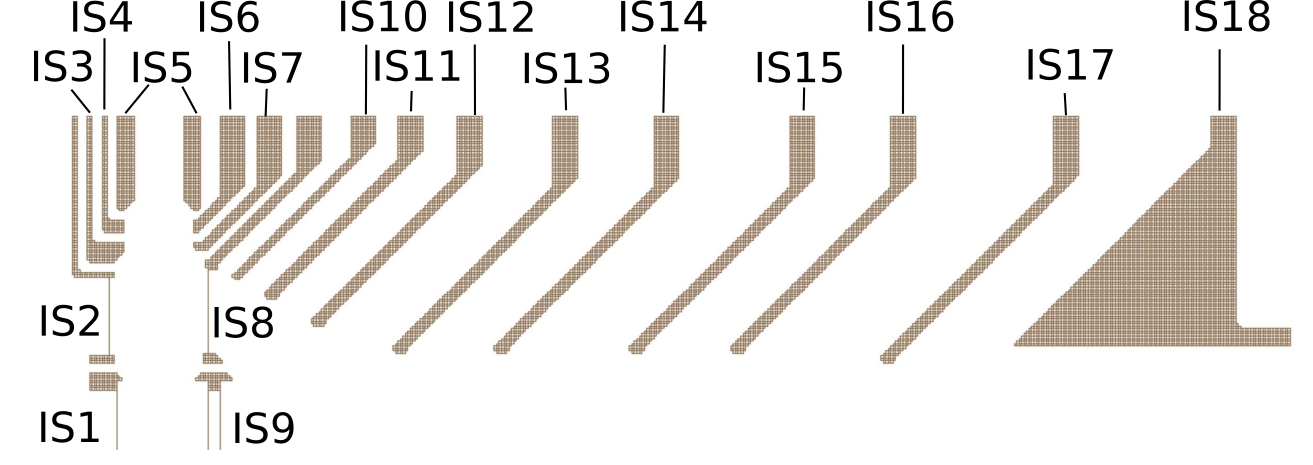
\includegraphics[width= 0.9\textwidth]{Setup/Proto_IS_sim.png}
			\caption{SIMION Model of the Ion-Source of the NIM Prototype \cite{Diss_Meyer}.}
			\label{fig:SetupProtoISSim}
		\end{figure}
		
		\begin{figure}[h]
			\centering
			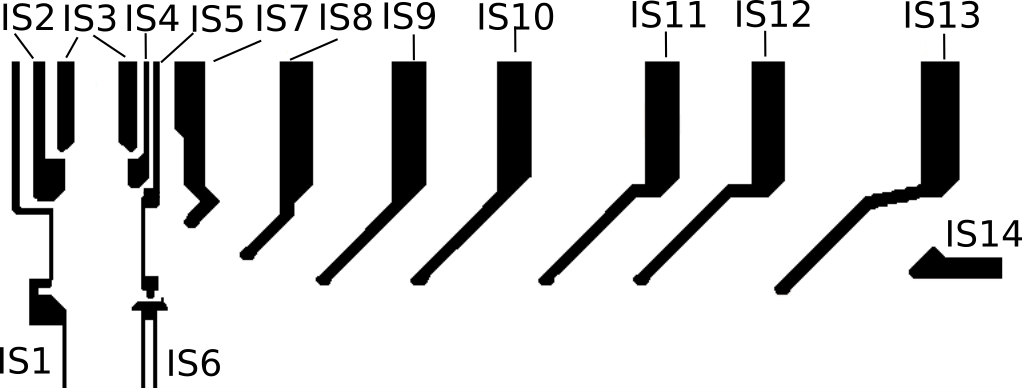
\includegraphics[width=0.9\textwidth]{Setup/ISFlight_bearb.png}
			\caption{SIMION Model of the Ion-Source of the NIM ProtoFlight Model.}
			\label{fig:SetupPFMISSim}
		\end{figure}
		\begin{figure}[h] % In Bild noch Fil 7/ Fil 4 durch IS5/ IS3 ersetzen.
			\begin{subfigure}{0.5\textwidth}
				\centering
				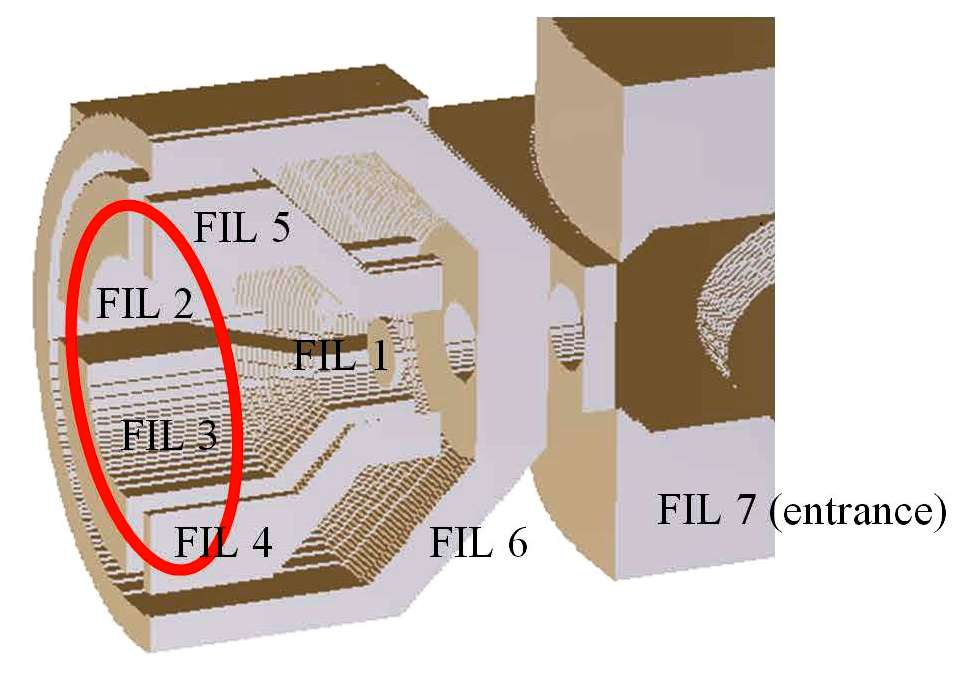
\includegraphics[width =0.85\textwidth]{Setup/Proto_FilEl_sim.jpg}
			\end{subfigure}
			\begin{subfigure}{0.5\textwidth}
				\centering
				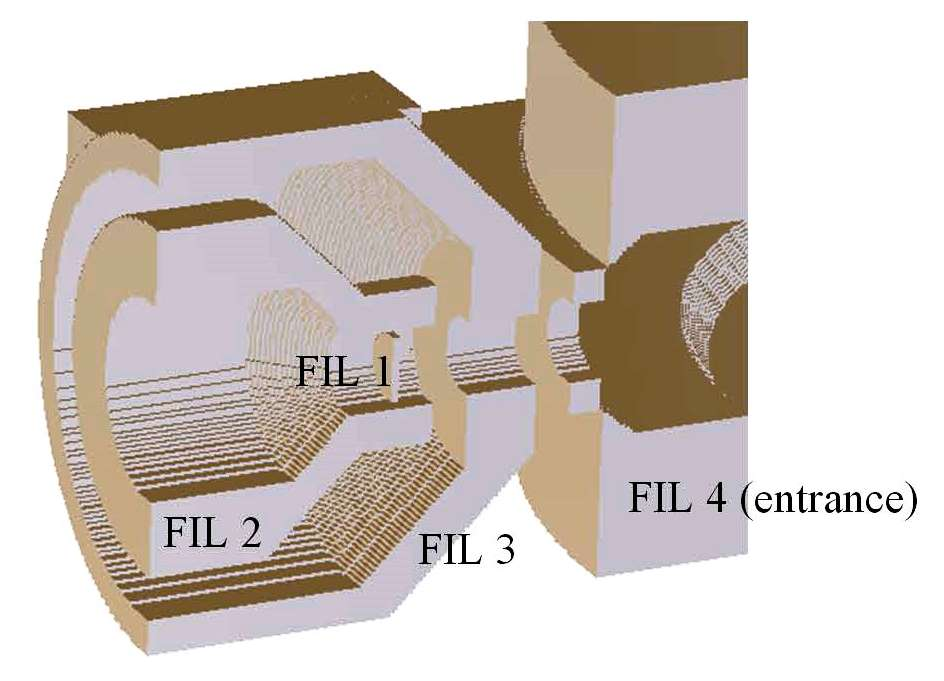
\includegraphics[width = 0.85\textwidth]{Setup/PFM_FilEl_sim.jpg}
			\end{subfigure}
			\caption{Left: Prototype filament housing. Right: PFM filament housing.}
			\label{fig:SetupFilElSim}
		\end{figure}

		\begin{figure}[h]
			\centering
			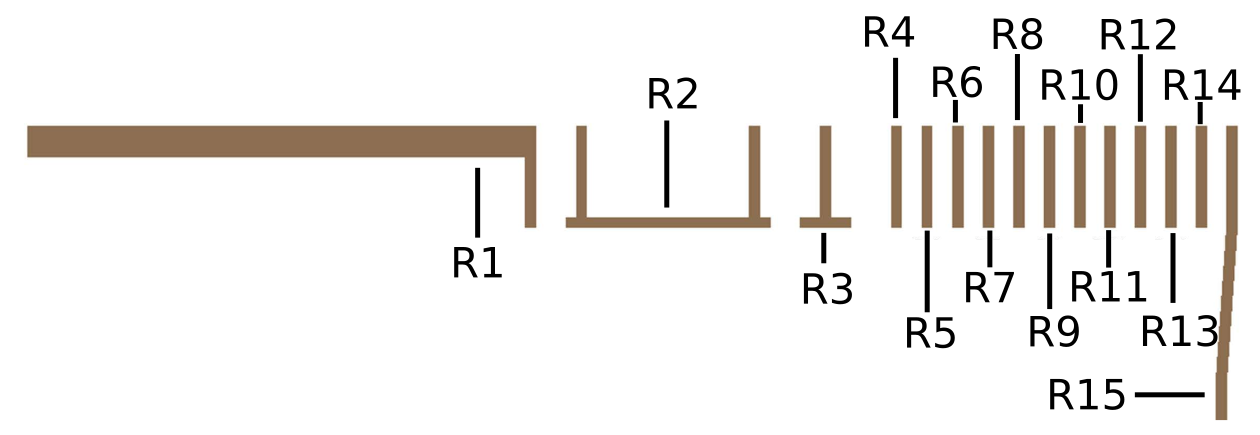
\includegraphics[width=0.9\textwidth]{Setup/Prototype_Reflectron_sim.png}
			\caption{SIMION Model of the ion-mirror of the NIM Prototype \cite{Diss_Meyer}.}
			\label{fig:SetupProtoReflSim}
		\end{figure}
		
		\begin{figure}[h] % Exchange reflectron through ion-mirror
			\centering
			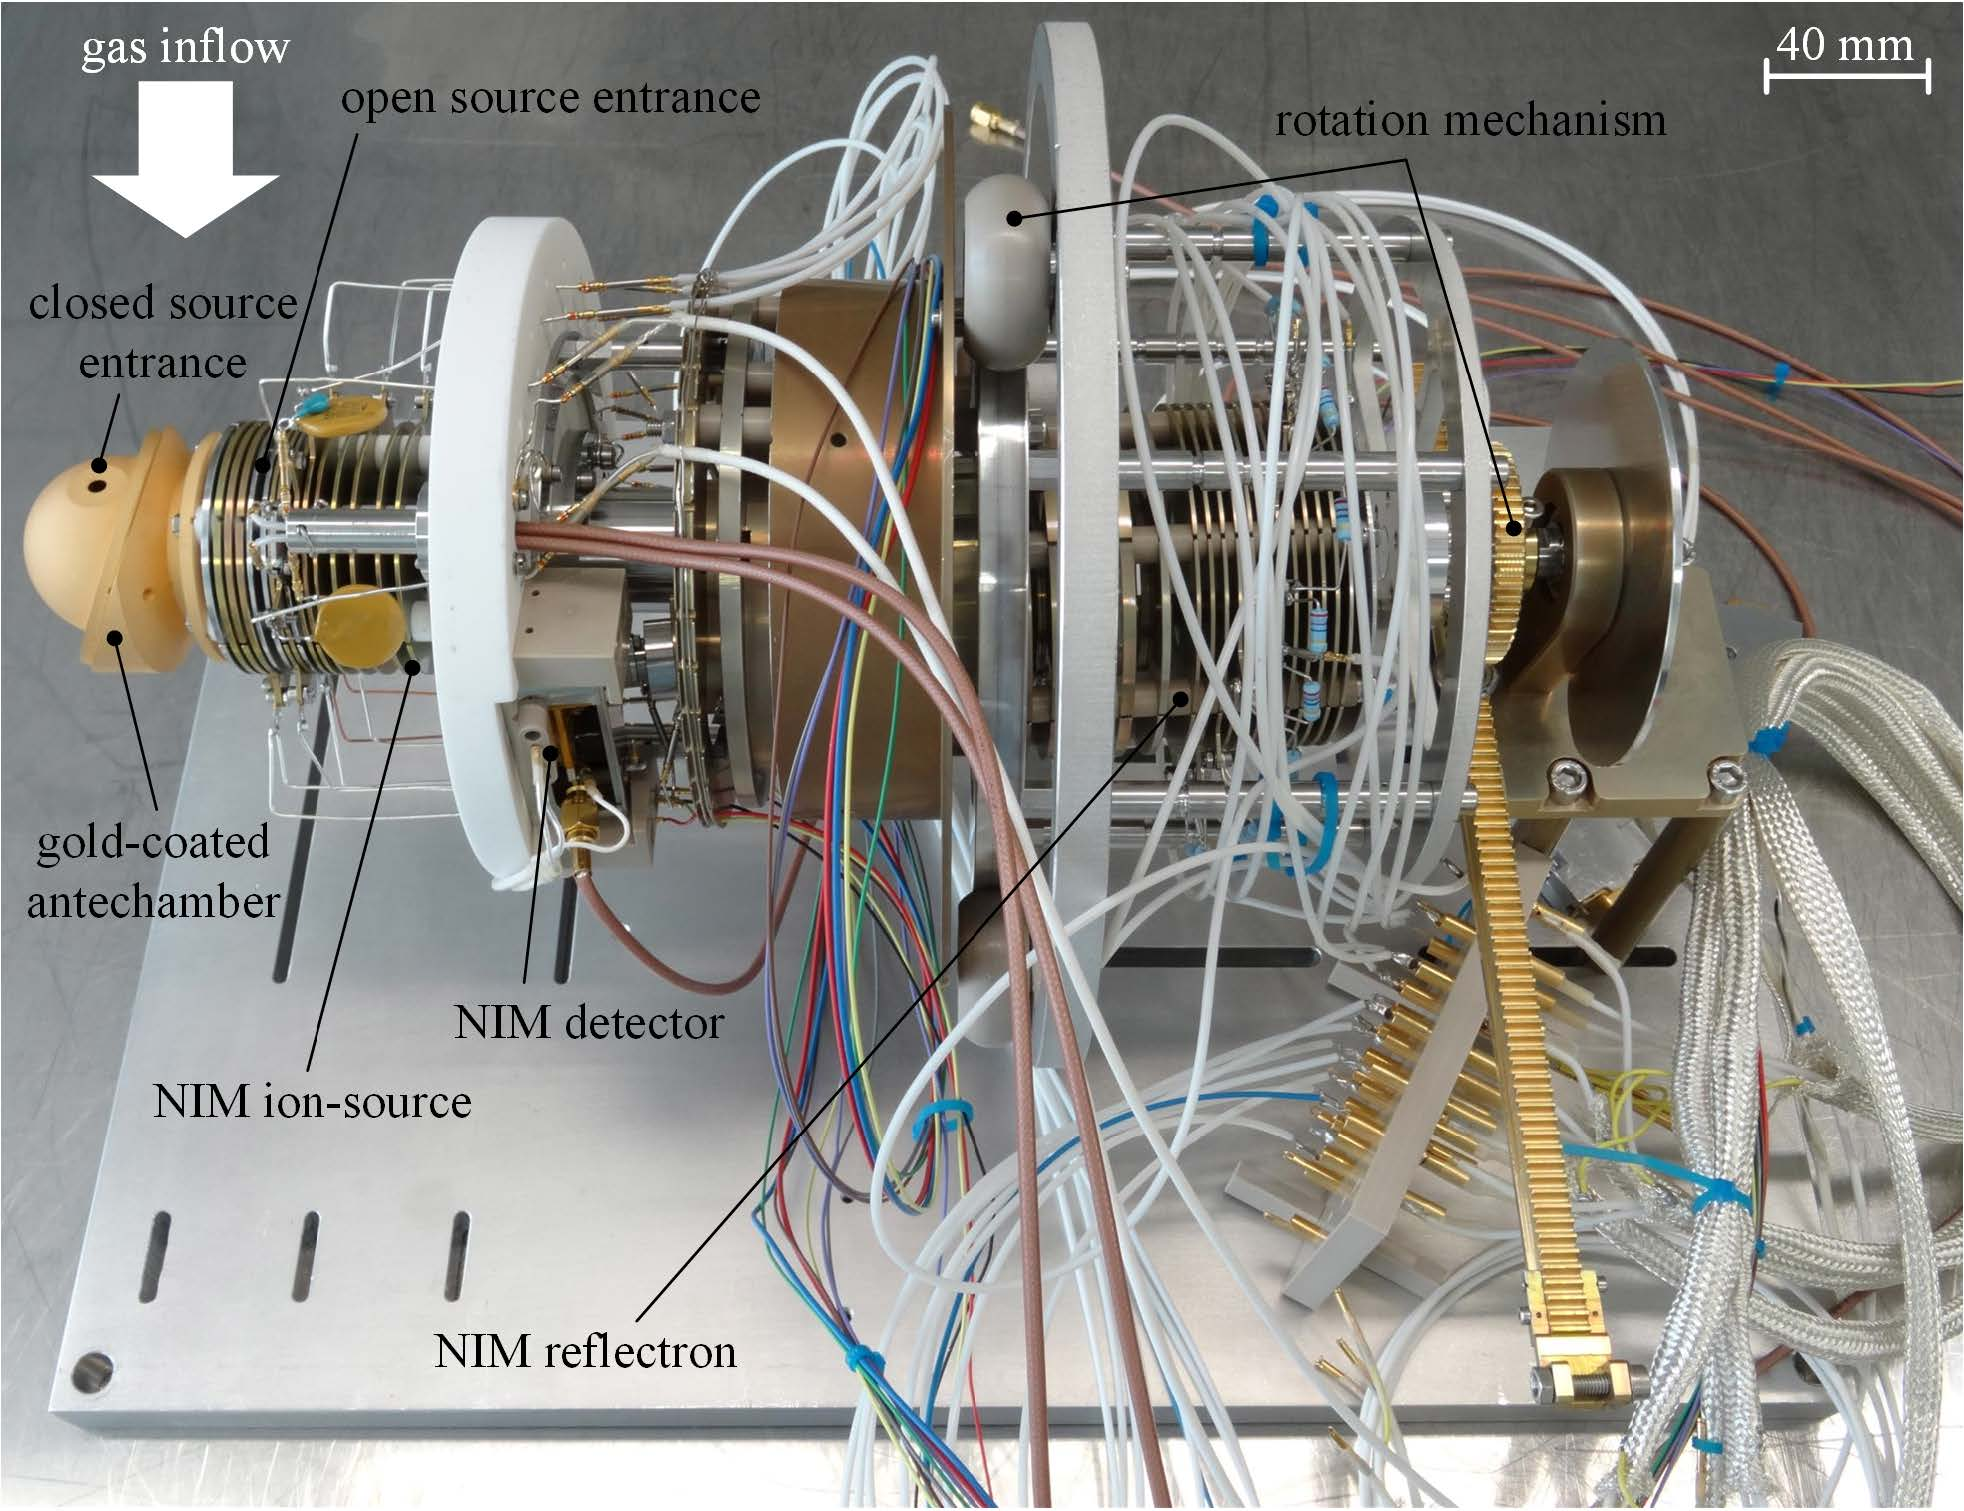
\includegraphics[width=\textwidth]{Setup/Prototype_totPic.jpg}
			\caption{NIM Prototype \cite{Diss_Meyer}.}
			\label{fig:SetupProto}
		\end{figure}
		\begin{comment}
			\begin{figure}[h] % Exchange picture through a picture collection (EGU2020 slid of the sensor in different states) Add a picture, where the inner parts are visible for comparison. Include a lineal ruler into the pictures.
				\centering
				\includegraphics[width=0.8\textwidth]{Setup/PFM_in_calib_Setup.JPG}
				\caption{NIM PFM sensor head in calibration setup.}
				\label{fig:SetupPFM}
			\end{figure}
		\end{comment}
		
			
%---------------------------------------------------------------------------------------------------------------

		\subsection{Detector \notes{Draft}}\label{subsubsec:SetFacPumpst} % May merge that chapter with the previous one.
		\begin{figure}[h] % Photograph of the Prototype an Flight detector.
			\begin{subfigure}{0.5\textwidth}
				\centering
				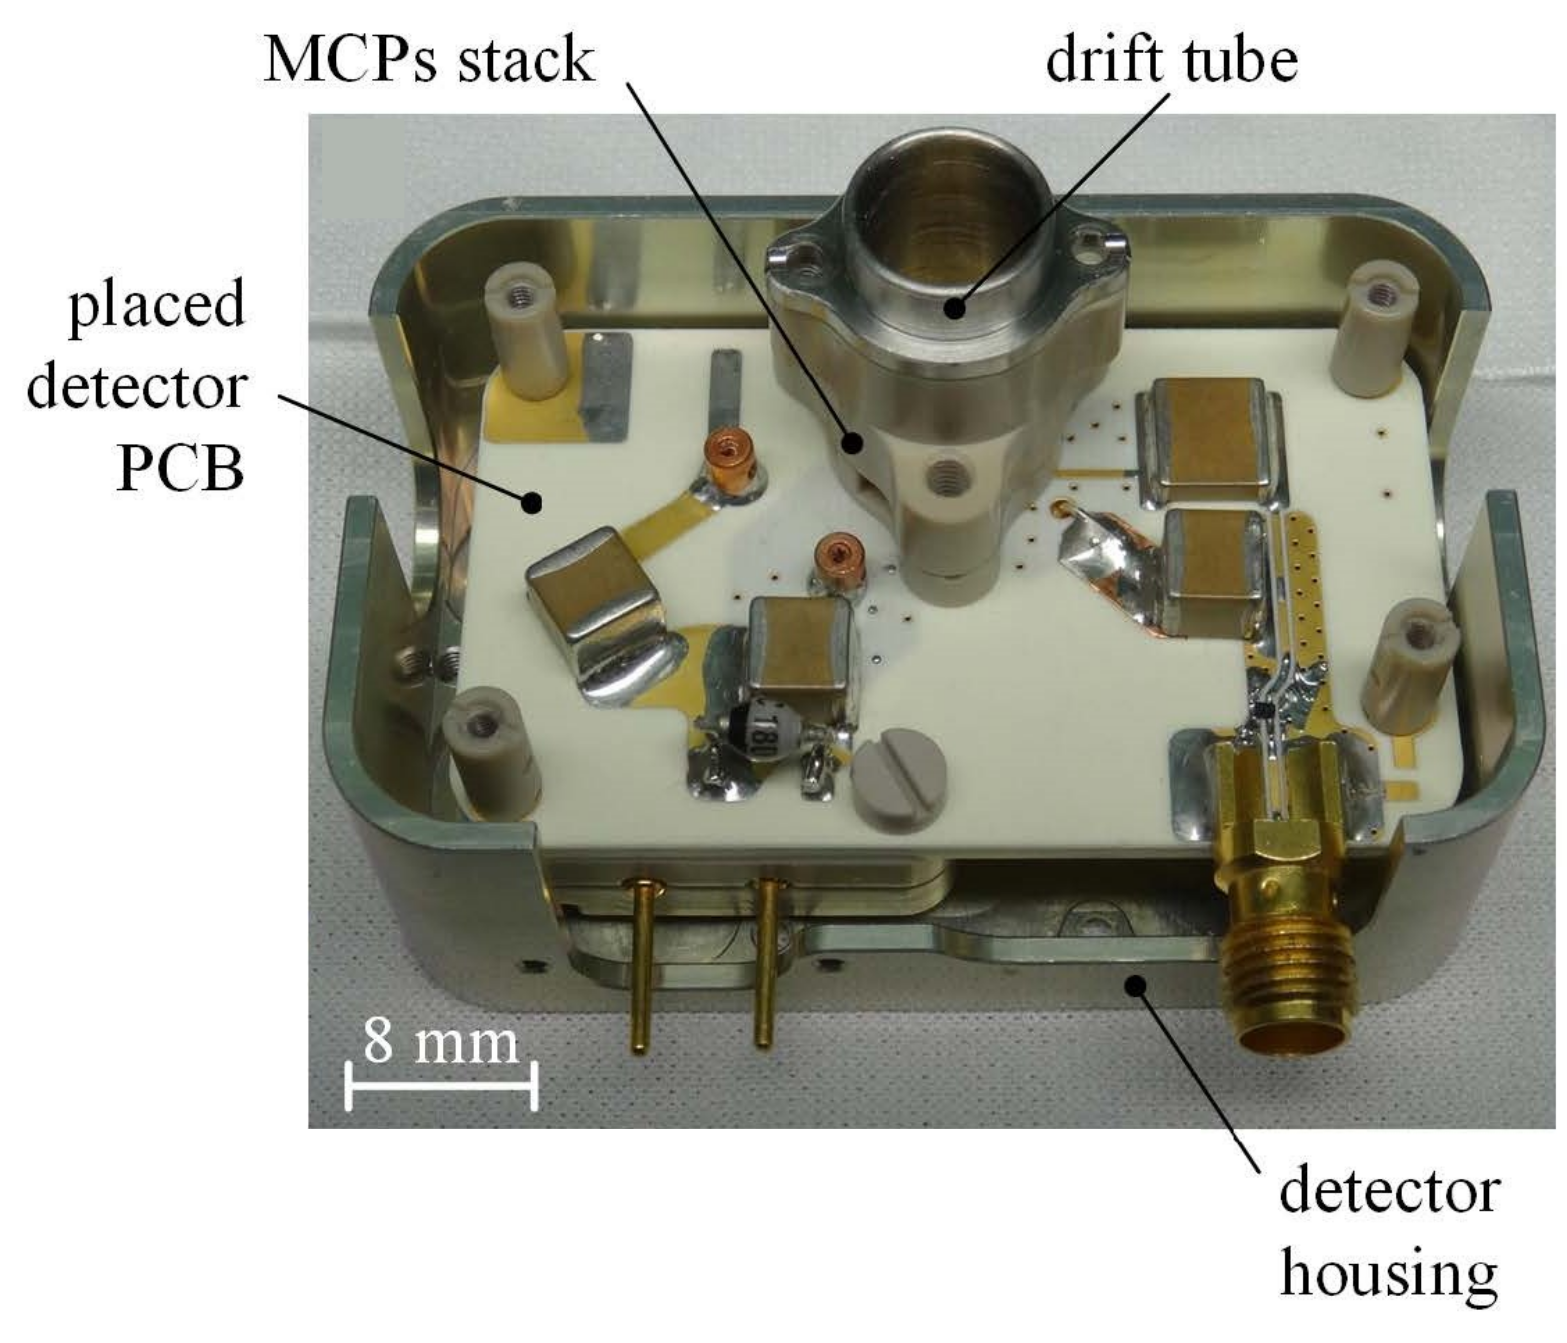
\includegraphics[width=\textwidth]{Setup/Prototype_Detector.png}
			\end{subfigure}
			\begin{subfigure}{0.5\textwidth}
				\centering
				\includegraphics[width=.9\textwidth]{Setup/Flight_Detector.png}
			\end{subfigure}
			\caption{Left: NIM Prototype detector \cite{Diss_Meyer}. Right: NIM Flight detector without its radiation shield.}
			\label{fig:DetPhotos}
		\end{figure}
		\begin{figure}[h] % Schematics of the 2 detector designs.
			\centering
			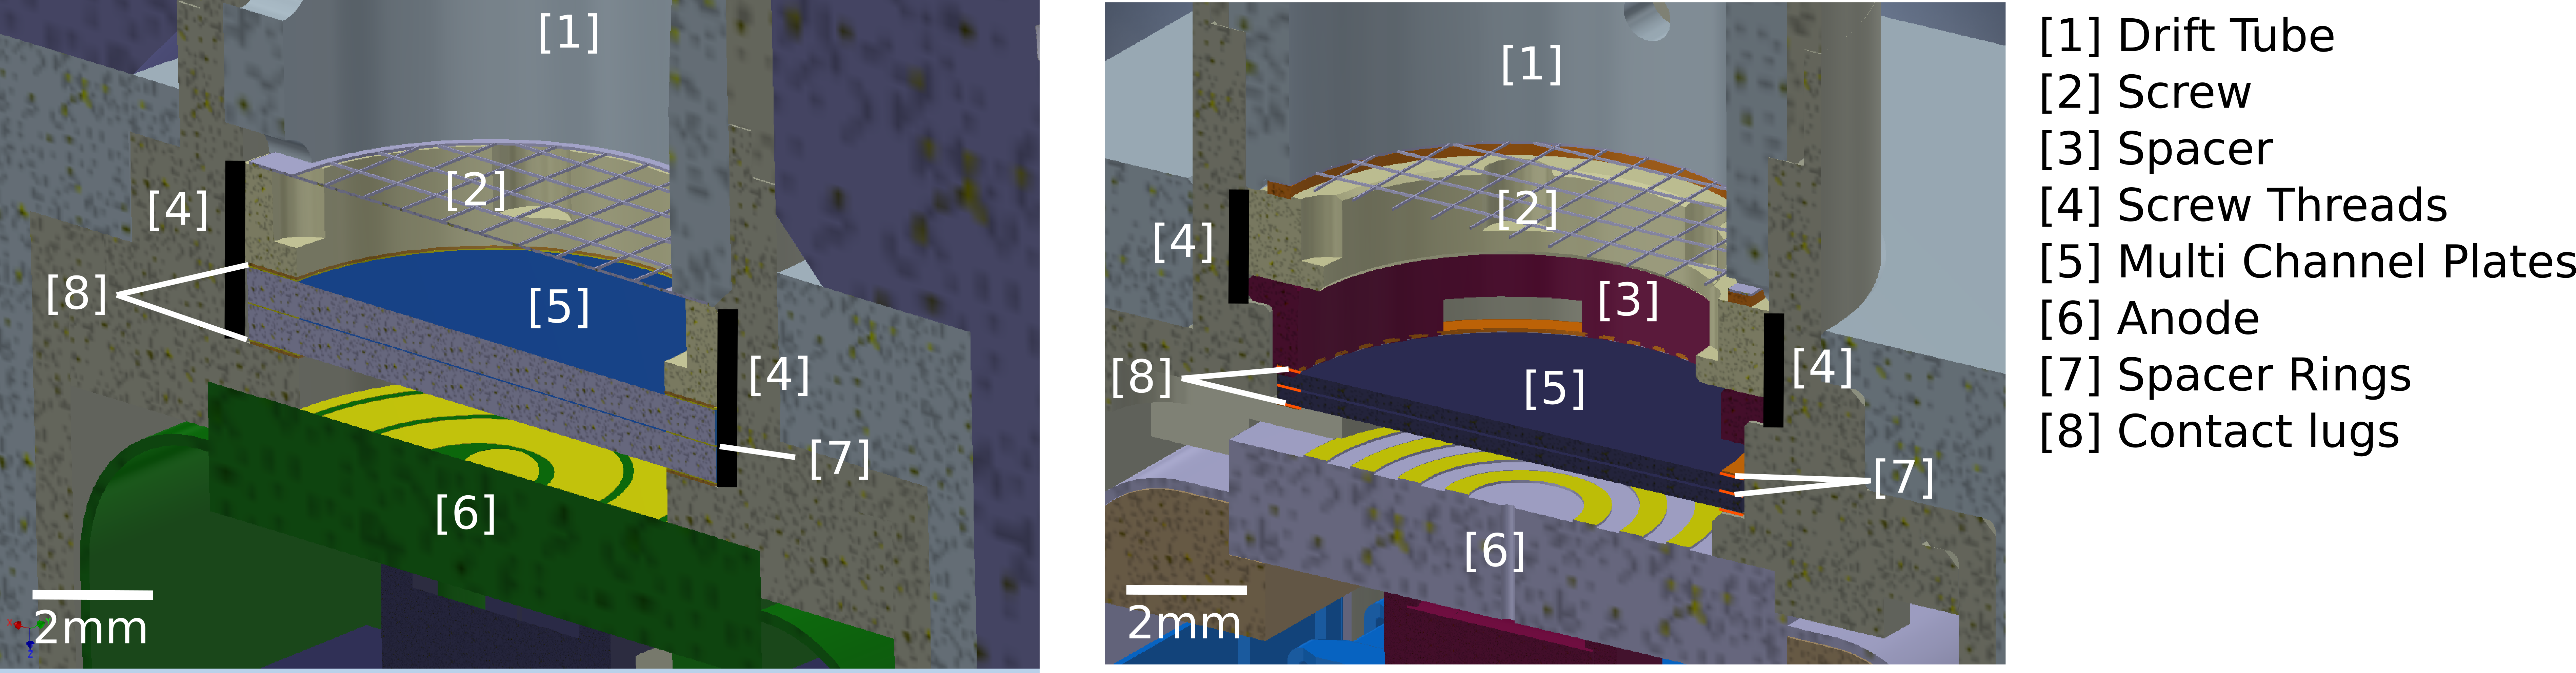
\includegraphics[width= \textwidth]{Setup/PFMDetectors.png}
			\caption{Schematics of the PFM detector housings. Left: preliminary design. Right: final flight design.}
			\label{fig:FlightDetSchemata}
		\end{figure}
		% free play = technisch Spiel. Put it in during proofreading.
		The NIM Prototype detector has a rigid Printed Circuit Board (PCB) on which the electrical components and the drift tube with the MCP stack are mounted (Fig.\,\ref{fig:DetPhotos}~left). Due to Jupiter's strong radiation field, the detector has to be shielded to reduce the noise level induced by the strong radiation and to increase the detector's lifetime. To minimized the required shielding mass, the flight detector has to be very compact. This was achieved by using a flex PCB to fold the detector into a peek housing (Fig.\,\ref{fig:DetPhotos}~right). Fig.~\ref{fig:FlightDetSchemata}~left shows the schema of a preliminary design of the peek housing containing the MCPs with the drift tube attached. The MCPs lay on a ledge 1~mm above the anode. A diode generates a voltage between the MCP backside and the anode to accelerate the electrons from the MCP backside towards the anode (cf. electrical schema Fig,\,\ref{fig:FlighElecSchema}). There are two contact lugs on top and at the bottom of the MCP stack to apply a voltage over the MCPs. The MCPs are fixed with a peek screw within the housing. In the old design, the screw threads were milled down to the ledge. When the MCPs were mounted, they often canted in the threads. In addition, it was not possible to determine, how much the screw had to be tightened. When the screw was tighten too much, the MCPs broke as they consist of lead glass and are therefore very fragile. When the screw was too loose, the two contact lugs had no reliable contact to the MCPs. When applying a high voltage over the whole MCP stack, the gaps between the contact lugs and the MCPs act as an additional resistors over which the voltage builds up resulting in a discharge between the electrodes and the MCPs. The discharge can propagate through the whole MCP stack and damages the readout electronics. As a consequence, the screw thread was milled less far and an additional mechanical stop was made to tighten the screw only down to that stop (Fig.\,\ref{fig:FlightDetSchemata}~right). This prevented the MCPs from canting in the screw thread thus it was not milled down to the bottom of the lower ledge and with the mechanical stop, the screw could not be tightened too much to break the MCPs. In addition, a peek space was added between the screw and the MCPs to push down the MCPs uniformly. Due to the tolerances in the manufacturing process of the different parts of the housing, metallic spacer rings are added between the peek spacer and the contact lug of the top MCP to close the resulting gap. The number of added rings varied between each detector because the gap is different for each manufactured housing. With this design, the contact between the MCPs and the contact lugs could be improved but from the electrical point of view its still not a clean electrical contact. To make the system more robust against discharges the Zener diode was exchanged through a resistor ($R_D$). The flight electronics sets the voltage $U_{stack}$ between the top MCP and the anode. The MCPs and the diode act as resistors, which are connected in series. Therefore, the potential drop over the MCPs depends on the potential drop over the diode. The voltage drop over a Zener diode is 180~V independent of $U_{stack}$. Therefore, the voltage over the MCPs $U_{MCP}$ is 180~V lower than $U_{stack}$. When having a resistor $R_D$ instead of a diode, the voltage over the MCPs cannot be calculated by just having $U_{stack}$ because the resistance of the MCPs $R_{MCP}$ depends on the voltage $U_{MCP}$ applied over them. It also changes with time due to ageing because the conductive material inside the MCP channels degrades over time. Therefore, the current $I_{MCP}$ flowing through the system has to be known to be able to calculate $U_{MCP}$. The NIM flight electronics is not designed to measure this current because it was designed for a detector with a diode where a current measurement would be unnecessary. With the laboratory electronics we did a calibration to determine the relationship between $U_{stack}$ and $U_{MCP}$ (Chap.~\ref{chapExp:Det}).\\
		In the following section, $U_{MCP}$ is derived as a function of the different voltages known when measuring with laboratory electronics. Fig.\,\ref{fig:FlighElecSchema} shows the circuit diagram of the detector when operated with laboratory electronics and Table\,\ref{tab:ElecSchemaVariableList} summarizes the used variables. The current flowing through the MCPs $I_{MCP}$ is measured with the resistor $R_M$:
		\begin{equation}
			I_{MCP} = \frac{U_{RM}}{R_{M}}
		\end{equation}
		With $U_{RM}$ the voltage over the resistor $R_{M}$ which is:
		\begin{align}
			U_{RM} &= U_{PSA} - U_{A}\\
				   &= U_{PSMCP} + U_{PSD} - U_A
		\end{align}
		With $U_{PSA}$ the power supply output voltage for the anode, $U_{A}$ the voltage applied on the detector anode, $U_{PSD}$ the power supply output voltage applied at the top contact lug of the MCP stack and $U_{PSMCP}$ the voltage difference between the two power supply outputs. $U_{PSMCP}$ is:
		\begin{equation}
			U_{PSMCP} = U_{RM} + 2\cdot U_{Ri} + U_{RD} + U_{MCP}
			\label{eq:UpsmcpTot}
		\end{equation}
		With $U_{Ri}$ the voltage over the input resistors $R_i$, which are there to damp noise coupled into the detector circuit from the power supply:
		\begin{equation}
			U_{Ri} = I_{MCP}\cdot R_i
		\end{equation} 
		$U_{RD}$ is the voltage over the resistor $R_D$ replacing the former diode. The current $I_A$ induced when an ion generates an electron avalanche, is very low compared to the current $I_{RD}$. Therefore, $I_{MCP} = I_{RD}$ and:
		\begin{equation}
			U_{RD} = I_{MCP}\cdot R_D
		\end{equation}
		Solving Eq.~\eqref{eq:UpsmcpTot} to $U_{MCP}$ and inserting the different voltages results in:
		\begin{align}
			U_{MCP} =& U_{PSMCP} - U_{RM} - 2\cdot U_{Ri} - U_{RD}\\
			=& U_{PSMCP} - U_{PSMCP} + U_{PSD} - U_A - 2\cdot I_{MCP} R_i - I_{MCP} R_D\\
			=& (U_A - U_{PSD})\cdot(1 + \frac{2R_i + R_D}{R_M}) - U_{PSMCP}\frac{2R_i + R_D}{R_M}
		\end{align}
		
		\begin{comment}
		% Pumpstand nr.~2 was used to perform stand-alone tests with the different NIM detectors. The test setup consists of a vacuum chamber, a HV power supply, an oscilloscope, a computer to remote control the oscilloscope and a HV meter (Fig.~\ref{fig:Pumpstand2}).		

		\begin{figure}[h]
			\begin{subfigure}{.5\textwidth}
				\centering
				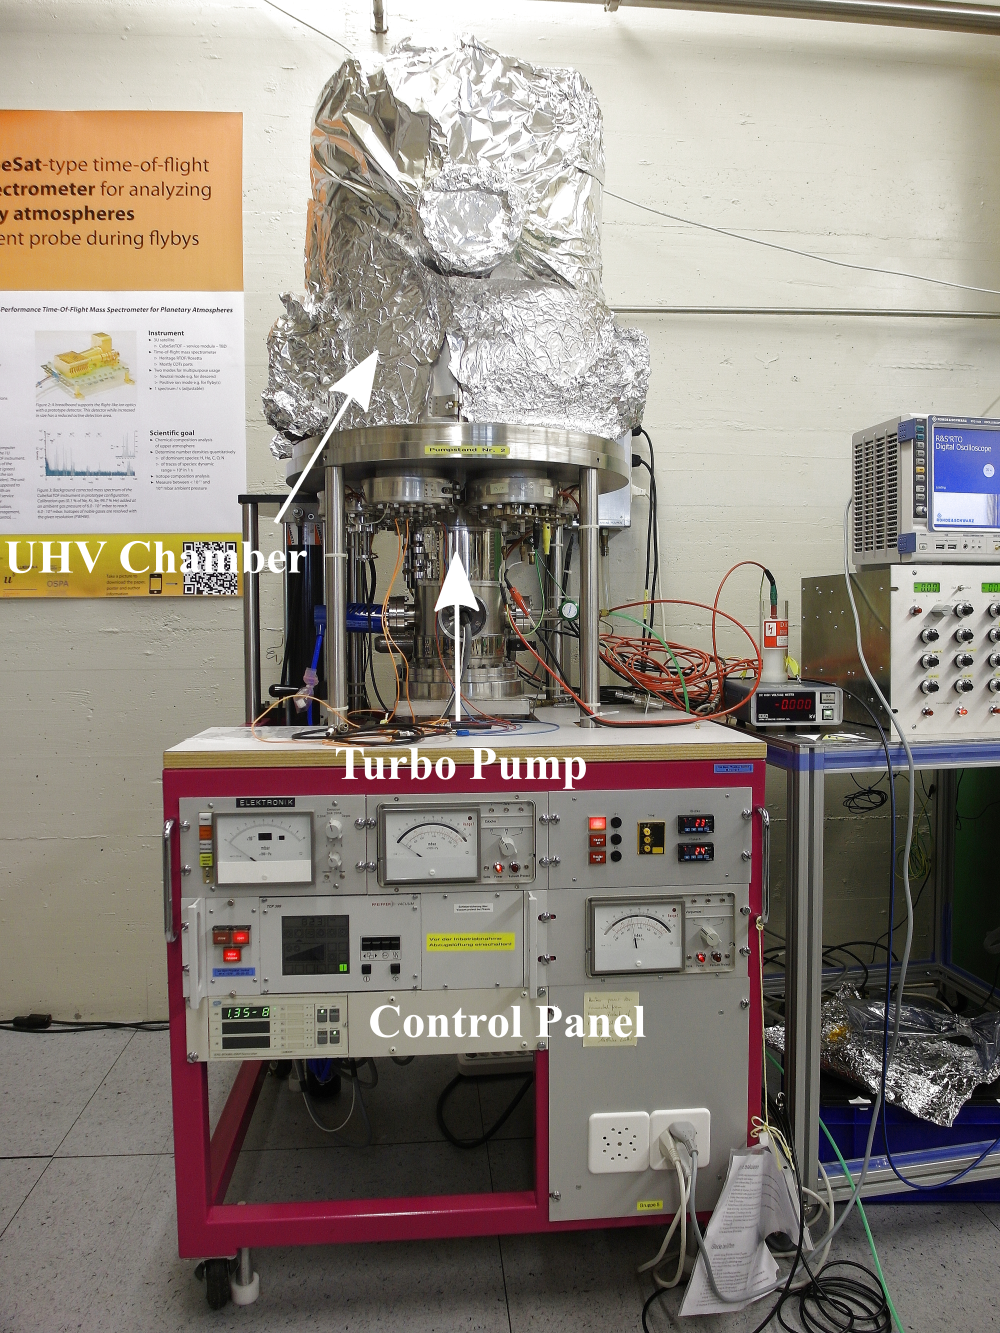
\includegraphics[width=0.8\textwidth]{Bilder/Galerie_Setup/Pumpstand2_midres.png}
			\end{subfigure}
			\begin{subfigure}{.5\textwidth}
				\centering
				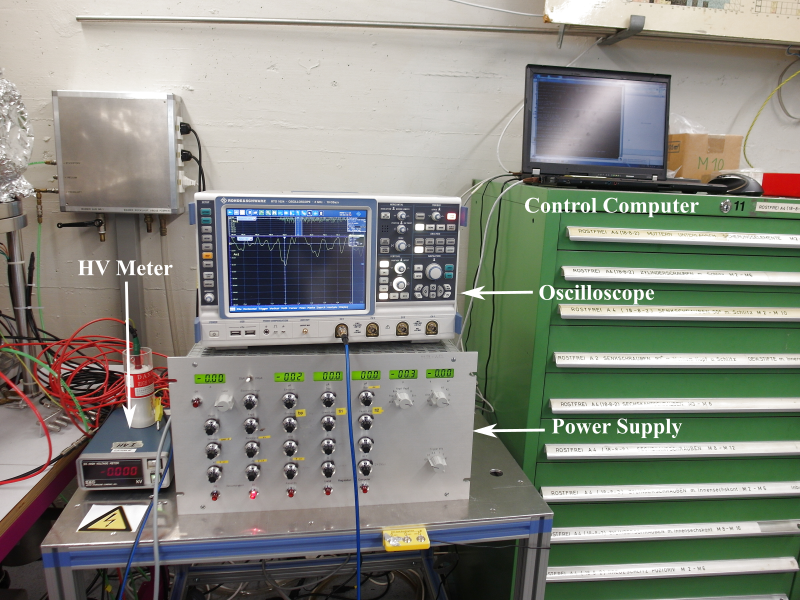
\includegraphics[width=\textwidth]{Bilder/Galerie_Setup/Pumpstand_PSOszi.png}
			\end{subfigure}
			\caption{Left: Pumpstand nr. 2. Right: Power supply, oscilloscope and control computer for the stand-alone tests of the detector. The signal on the oscilloscope is a noise signal.}
			\label{fig:Pumpstand2}
		\end{figure}
		\end{comment}
	
		\begin{figure}[h]
			\centering
			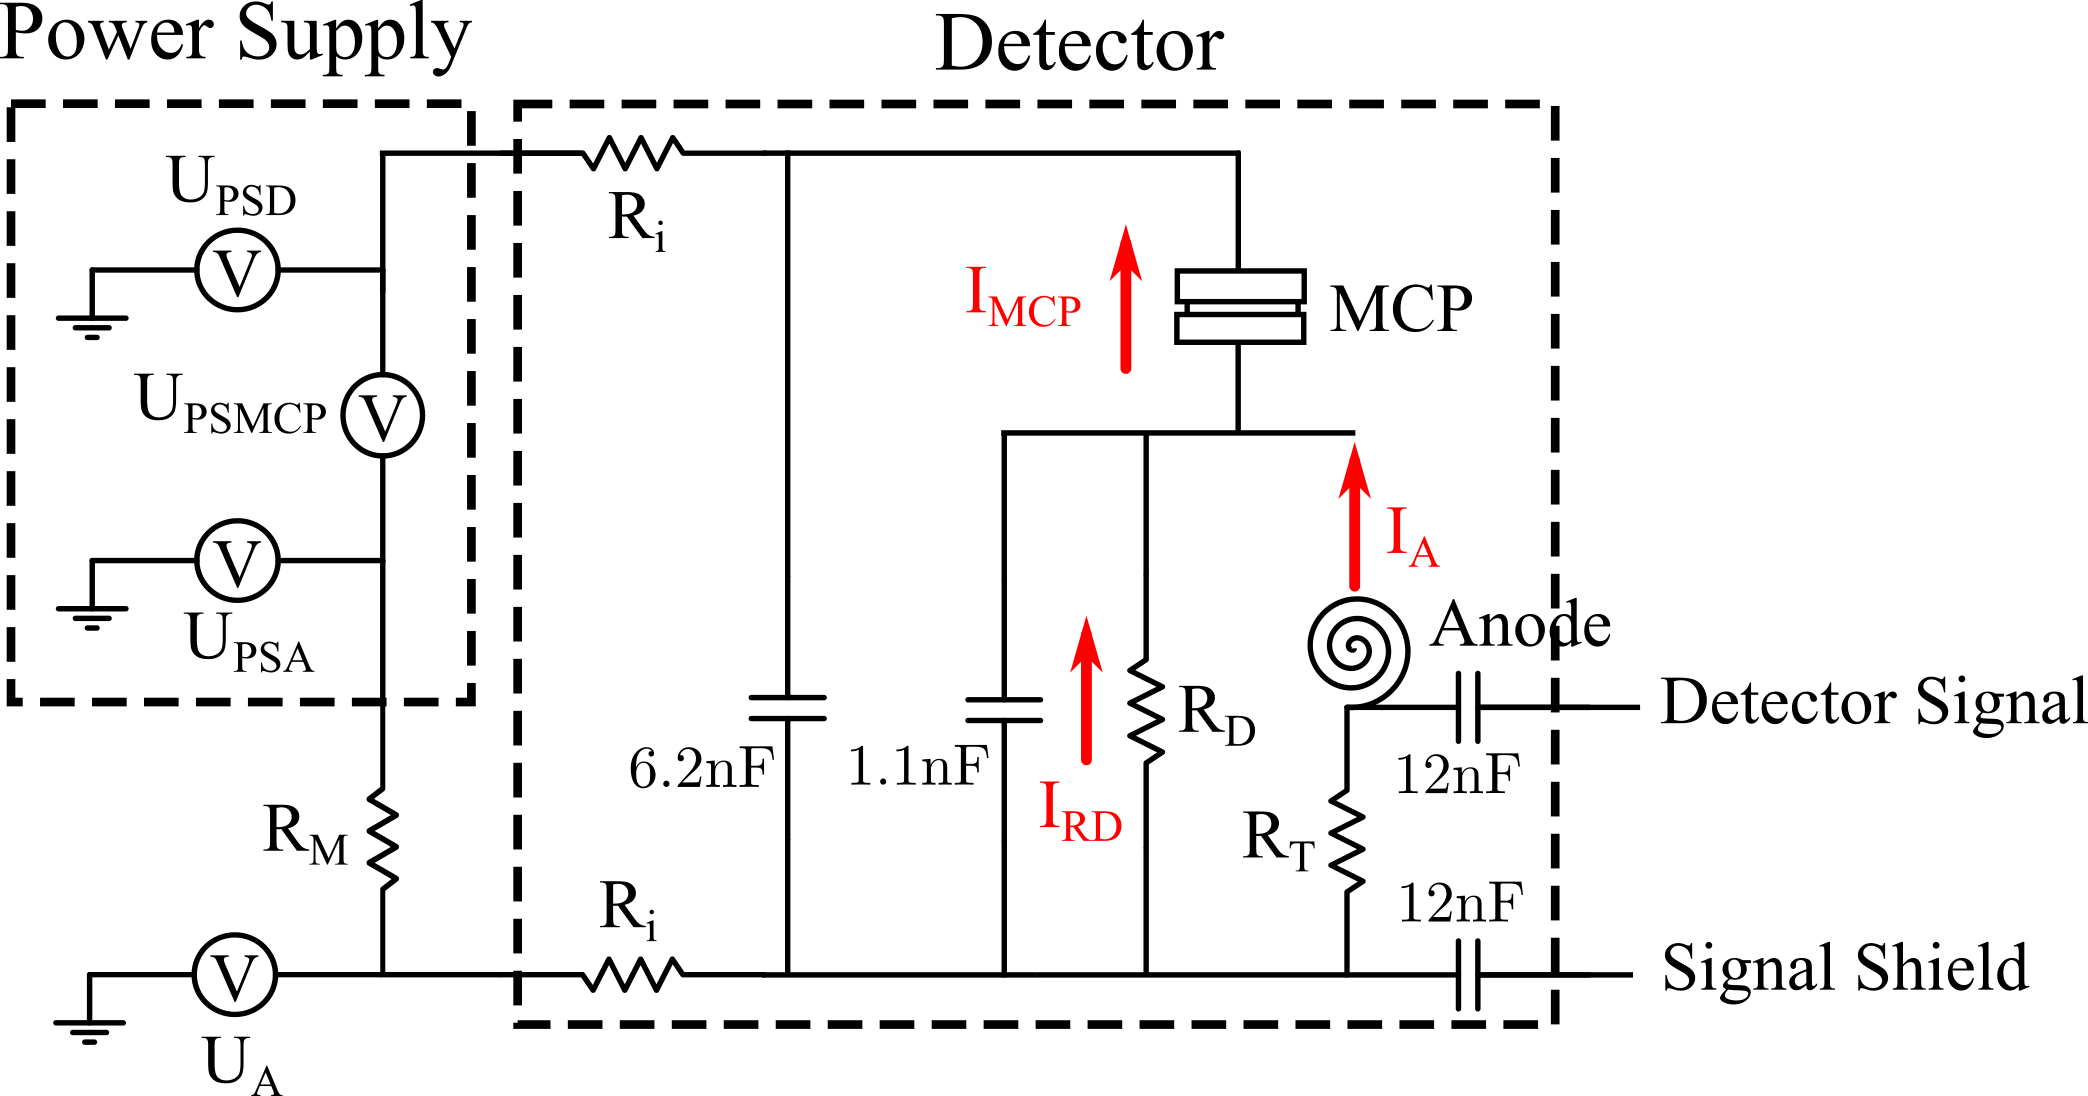
\includegraphics[width = .8\textwidth]{Bilder/Detector_elec_schema.png}
			\caption{Electrical schematics of the NIM flight detector with laboratory electronics attached.}
			\label{fig:FlighElecSchema}
		\end{figure}
		
		
		\begin{table}[h]
			\begin{center}
			\begin{tabular}{|m{1.5cm}|m{5.4cm}|m{1.5cm}|m{5.4cm}|}
				\hline
				R\textsubscript{D}& Resistor replacing the former diode & U\textsubscript{A}& Voltage on the detector anode \\
				R\textsubscript{i} & Detector input resistor & U\textsubscript{MCP}& Voltage over the MCPs \\
				R\textsubscript{M}& Resistor used to determine I\textsubscript{MCP} &U\textsubscript{PSA} & Anode voltage output of power supply \\
				R\textsubscript{MCP}& MCP resistance & U\textsubscript{PSD} & Drift voltage output of power supply \\
				R\textsubscript{T} & 50\,$\Omega$ termination & U\textsubscript{PSMCP} & Voltage difference  between U\textsubscript{PSA} and U\textsubscript{PSD} \\
				I\textsubscript{A} & Current induced in the MCPs when an ion hits the MCPs & U\textsubscript{RD}& Voltage over R\textsubscript{D} \\
				I\textsubscript{ion} & Ion current hitting the MCPs & U\textsubscript{Ri}& Voltage over R\textsubscript{i} \\
				I\textsubscript{MCP} & Current flowing through the MCPs &U\textsubscript{RM}& Voltage over test resistor R\textsubscript{M}\\
				I\textsubscript{RD} & Current flowing through R\textsubscript{D} &&\\
				\hline
			\end{tabular}
			\end{center}
			\caption{Variable list for the detector.}
			\label{tab:ElecSchemaVariableList}
		\end{table}
	

		\begin{comment}
		\begin{table}
		\begin{tabular} {l | r | l}
			\hline
			Variable & Value & Description\\
			\hline
			U\textsubscript{PSD} & -2500 V & Drift voltage at the output of the power supply\\ % useless maybe
			U\textsubscript{PSMCP} & variable & Voltage difference between the two output channels of the power supply (phi)\\
			U\textsubscript{A} & variable & Detector anode voltage at the input\\
			$\varphi_{PSD}$ & -2500 V & Potential of the drift voltage at the output of the power supply\\
			$\varphi_{PSA}$ & variable & Potential of the anode at the outp of the power supply\\
			R\textsubscript{t} & 50 \si{\ohm} & terminating resistor\\
			R\textsubscript{A} & variable & equivalent resistance between MCP output and anode.\\
			R\textsubscript{i} & 100 \si{k\ohm} & Detector input resistance to damp noise coupled into the system by the super supply voltage line.\\
			I\textsubscript{A} & variable & Signal current produced by an ion triggering an electron avalanche in the MCPs\\
			\hline
		\end{tabular}
		\caption{Detector variables.}\label{tab:detVar}
		\end{table}
		\end{comment}
		
	
		%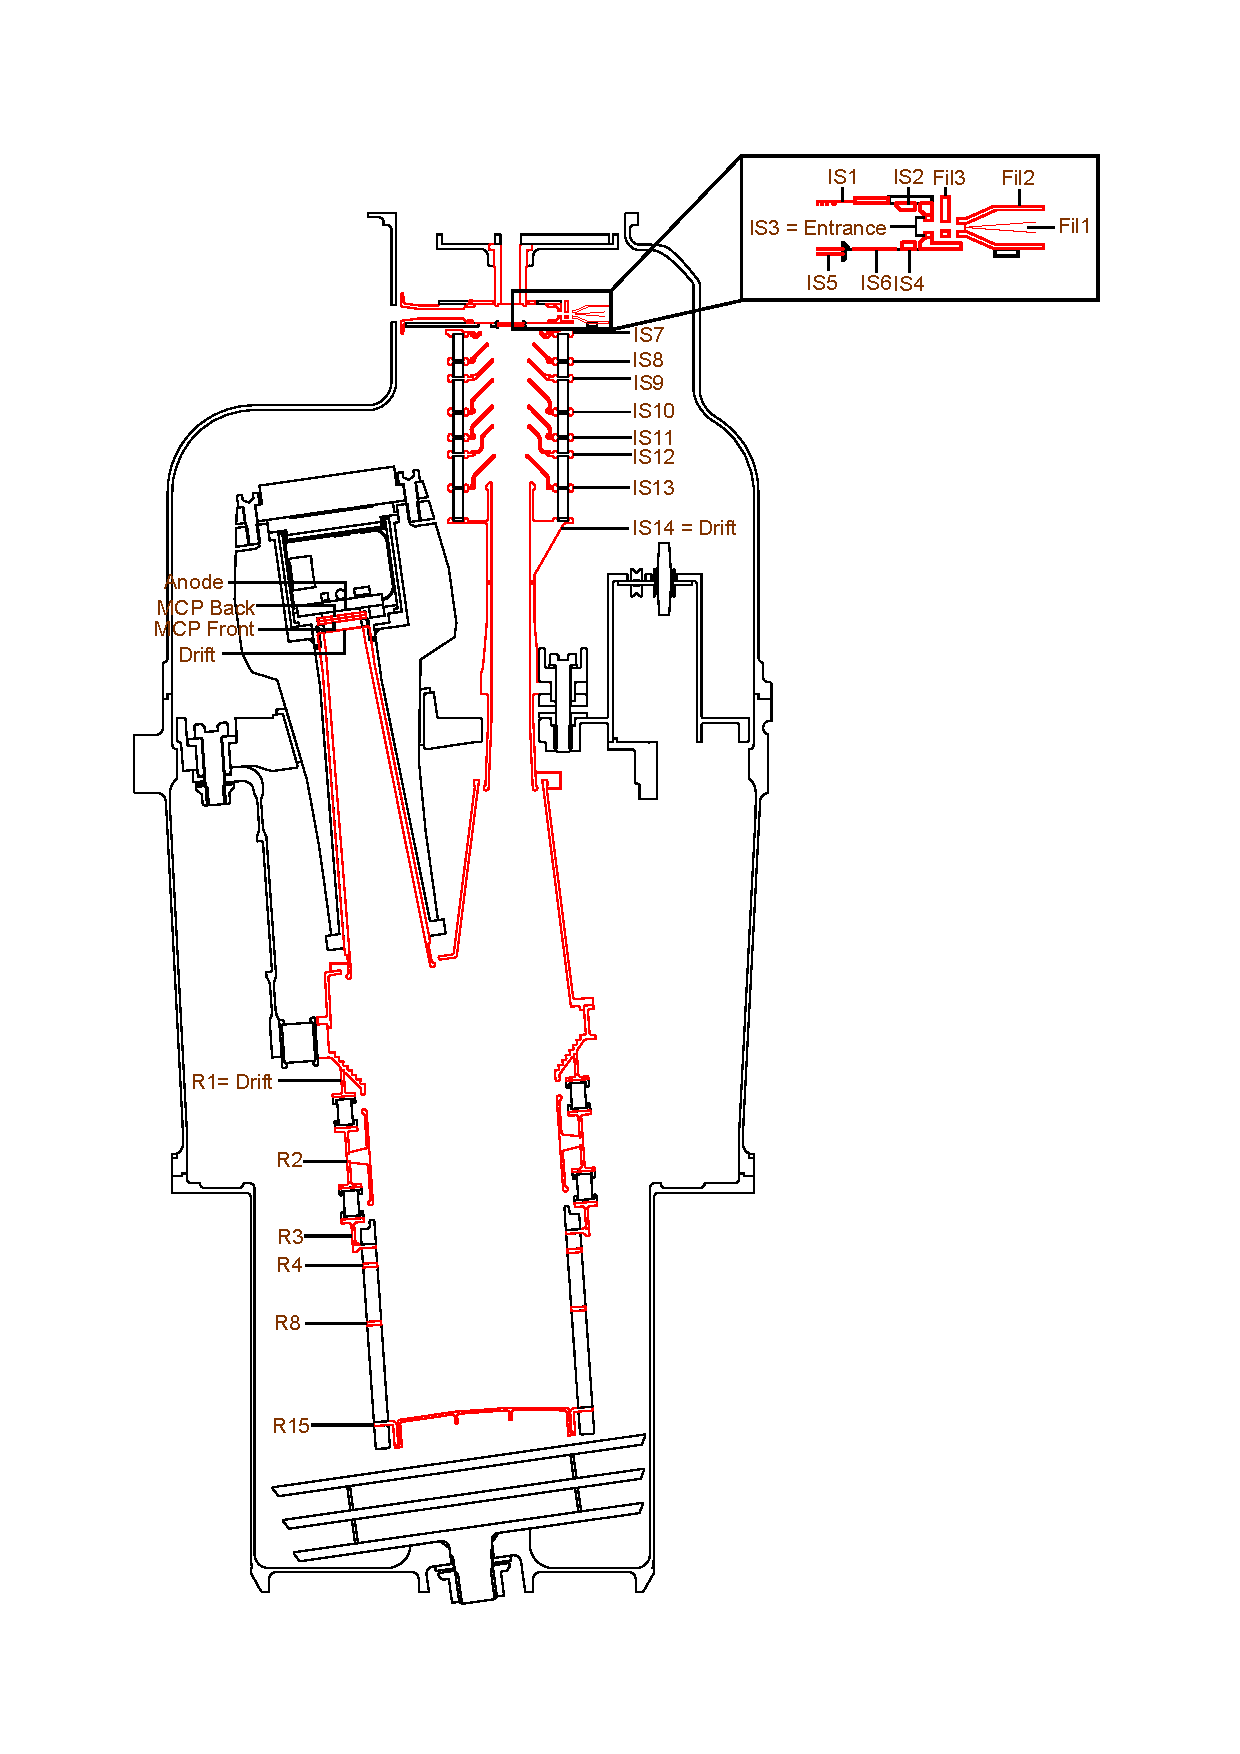
\includepdf[pages=-]{Setup/NIM_schema.pdf}
		\begin{figure}[h!]
			\centering
			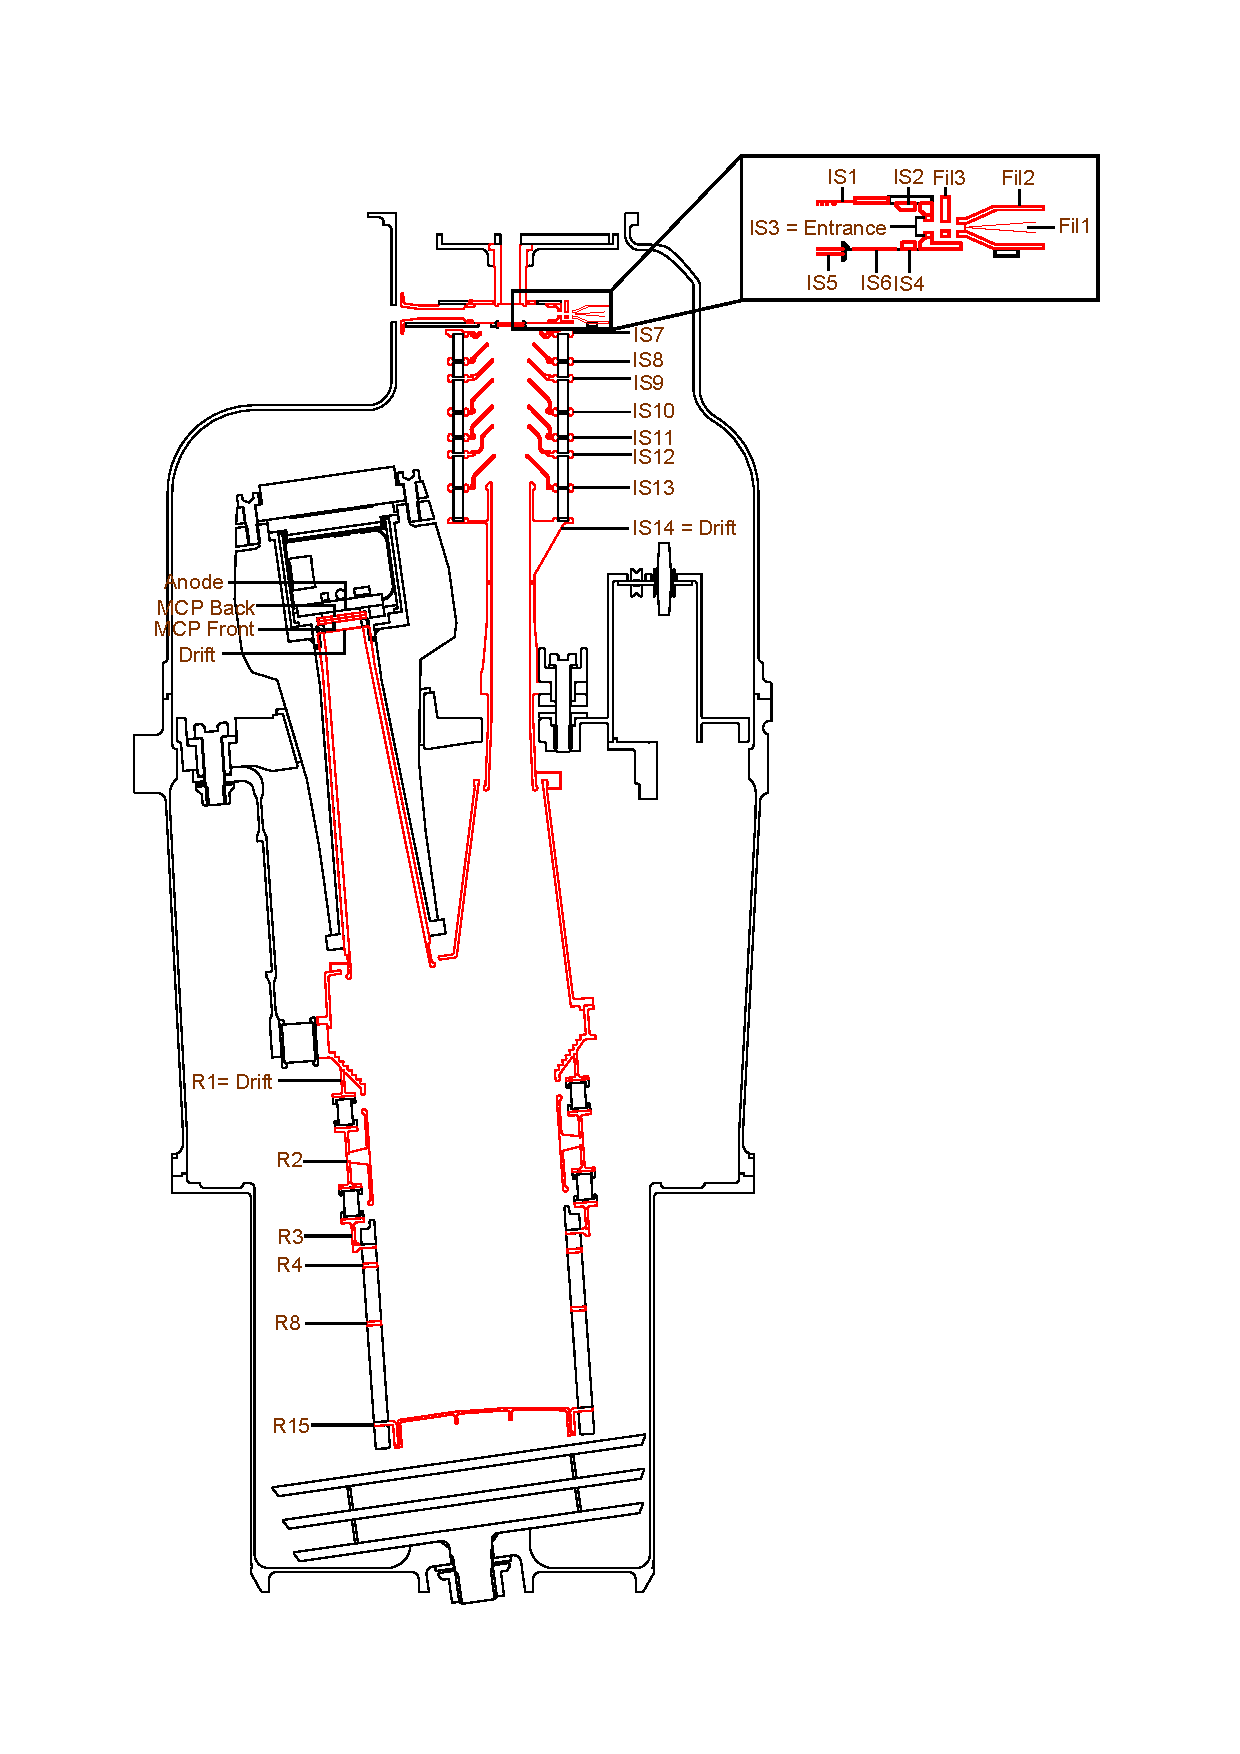
\includegraphics[width= 0.95\textwidth]{Setup/NIM_schema.pdf}
			\caption{Schematics of NIM flight design with all electrodes marked in red.}
			\label{fig:MINPFMTot}
		\end{figure}
	
	
	
